\documentclass[12pt,a4paper]{article}
\usepackage[utf8]{inputenc}
\usepackage[english]{babel}
\usepackage{acronym}
\usepackage{amsmath}
\usepackage{amsfonts}
\usepackage{amssymb}
\usepackage{algorithm}
\usepackage{algorithmicx}
\usepackage{algpseudocode}
\usepackage{tabularx}
\usepackage{multirow}
\usepackage{graphicx}
\usepackage{cite}
\usepackage[left=2cm,right=2cm,top=2cm,bottom=2cm]{geometry}
%\usepackage[headsepline, manualmark]{scrlayer-scrpage}
%\clearpairofpagesstyles


\makeatletter
\def\fps@figure{htbp}
\makeatother

\usepackage{setspace}
\onehalfspacing

\author{\\Research Project\\ \\Thomas Schick\\Florian Soulier\\ \\ Institute for Information Technology\\
Cologne University of Applied Sciences}
\title{Modern Reinforcement Learning Algorithms playing StarCraft II}
\begin{document}
\noindent
% \maketitle
\begin{titlepage}

    \newcommand{\HRule}{\rule{\linewidth}{0.5mm}} % Defines a new command for the horizontal lines, change thickness here
    
    \center % Center everything on the page
    
    %----------------------------------------------------------------------------------------
    %	LOGO SECTION
    %----------------------------------------------------------------------------------------
    \begin{flushright}
    % 
\includegraphics{./Figures/th_koeln_logo.pdf}\\[1cm] 
    % Include a department/university logo - this will require the graphicx package
    \end{flushright}
    \vspace{1.5cm}
    %----------------------------------------------------------------------------------------
    %	HEADING SECTIONS
    %----------------------------------------------------------------------------------------
    
    \textsc{\LARGE Technical University Cologne}\\[1.5cm] % Name of your university/college
    \textsc{\Large Research Project}\\[0.5cm] % Major heading such as course name
    
    %----------------------------------------------------------------------------------------
    %	TITLE SECTION
    %----------------------------------------------------------------------------------------
    
    \HRule \\[0.4cm]
    { \huge \bfseries
       Modern Reinforcement Algorithms playing StarCraft II }\\[0.4cm] % Title of your document
    \HRule \\[1.5cm]
     
    %----------------------------------------------------------------------------------------
    %	AUTHOR SECTION
    %----------------------------------------------------------------------------------------
    
    \begin{minipage}{0.4\textwidth}
    \begin{flushleft} \large
    \emph{Author:}\\
    Thomas \textsc{Schick\\} % Your name
    \end{flushleft}
    \end{minipage}
    ~
    \begin{minipage}{0.4\textwidth}
    \begin{flushright} \large
    \emph{
    Supervisor:} \\
    Prof. Dr. Beate \textsc{Rhein} \\ % Supervisor's Name
    \end{flushright}
    \end{minipage}\\[9cm]
    
    % If you don't want a supervisor, uncomment the two lines below and remove the section above
    %\Large \emph{Author:}\\
    %John \textsc{Smith}\\[3cm] % Your name
    
    %----------------------------------------------------------------------------------------
    %	DATE SECTION
    %----------------------------------------------------------------------------------------
    {\large Computer Science \& Engineering} \\
      {Faculty of Information, Media and Electrical Engineering}\\[2cm]
    {\large \today}\\[2cm] % Date, change the \today to a set date if you want to be precise
    
    
    \vfill % Fill the rest of the page with whitespace
    
    \end{titlepage}
\pagenumbering{Roman}
\newpage
\tableofcontents{}
\newpage
\section*{List of abbreviations}
%\addcontentsline{toc}{section}{abbreviations}
\begin{acronym}[Bash]
    \acro{API}{Application Programming Interface}
    \acro{AWS}{Amazon Web Services}
    \acro{CSV}{Comma Separated Values}
    \acro{ERP}{Enterprise Resource Planning}
    \acro{GCP}{Google Cloud Platform}
    \acro{IaaS}{Infrastructure as a Service}
    \acro{PaaS}{Platform as a Service}
    \acro{SaaS}{Software as a Service}
    \acro{SKU}{Stock-Keeping Unit}
\end{acronym}
\newpage
\pagenumbering{arabic}
\section{Introduction} 
When talking about artificial intelligence the most brought up topics often are recognition of images or sound based on vast amounts of correctly labeled data.
These technology rely heavily on human input to label the data in order for the machine learning algorithm to learn on.
The ability to learn abstract concepts however, differs strongly from the sheer memorizing of certain values in a pixels greyscale brightness.
This ability to learn is arguably one of, or even the most crucial aspect of human intelligence. And this is where reinforcement learning comes into play.
In this field of artificial intelligence, we attempt to guide an agent by supervisory signals in the form of rewards and penalties to learn an optimal behavior.
In the recent past a lot of milestones for reinforcement learning have been reached. The researchers at DeepMind as-well as @TODO
This work is motivated by the leaping steps the technology has made.
We adjusted the scope of the problem to a something we thought to be reasonable when considering the time and resources available for this research project. 
This project contributes to to deep reinforcement learning research by assessing hyper-parameters and models to state-of-the-art algorithms.
\section{Artificial Neural Networks}
This section describes the basics of simple neural networks. Since biological neural networks are the role model for the structure of so called artificial neural networks (ANN), some information about them will be presented first.
Following up with an overview on the internal functionality of artificial neurons, the smallest component of ANNs.
In order to store large amounts of information, such as memories of events, artificial neural networks can be used. Their structure and functions are modeled on those of biological neural networks, however greatly simplified.
Artificial neural network can be regarded an equivalent model to the Turing machine, regarding computability.
\subsection{The Biological Paradigm}
The mammal brain combined with the nervous system and it's capabilities in information processing serve as an archetype for today's artificial neural networks\cite{Rojas1996}
The fundamental components of such biological systems are neurons, complex and very small cells, which react to electrochemical signals.
The human nervous system, for example, consists of up to $10^{12}$ interconnected neurons.
Although, there are different types of neurons they share some basic characteristics. As shown in \ref{fig:neuron_schemantic} a neuron consists of a cell body with the nucleus, dendrites to receive stimuli of other cells and an axon ending with synapses used to pass on an electrical signal \cite{Patterson1997}.
\begin{figure}
    \centering
    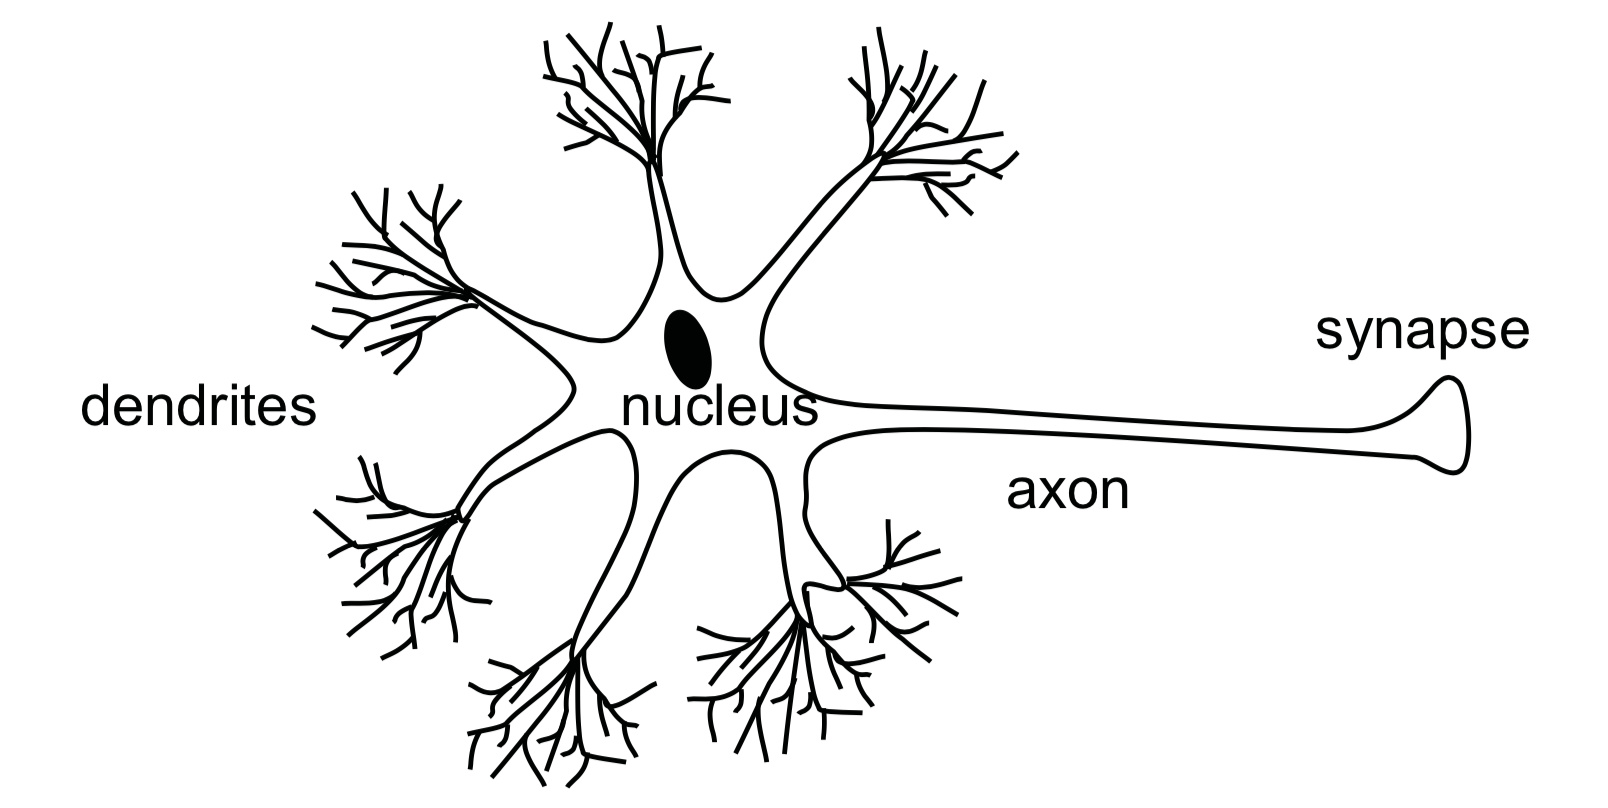
\includegraphics[width=0.5\linewidth]{Figures/Neuron_schemantic_depiction.png}
    \caption{Schematic depiction of a neuron}
    \label{fig:neuron_schemantic}
\end{figure}
A neuron receives electrochemical stimuli from other neurons or receptors, which act as biological sensors.
As a result of stimulation, the neuron fires a short sequence of electrical pulses via the axon to the synapses in order to stimulate other neurons or actor cells like the muscles. One single neuron can be connected to a thousand other neurons. Due to different types of synapses the signals at the transition can either be amplified or weakened \cite{Patterson1997}.
Nowadays the synapses in the neural network are seen as the main storage for information, so considered to be the main location of knowledge\cite{Rojas1996}.
\subsection{Artificial Neurons}
After a crude explanation of the biological mechanisms inside a neuron, we will now have a look at the technical imitation. A simple model of an artificial neuron also denoted as a processing unit can be seen as a three-stage system with multiple inputs and one single output (see fig.\ref{fig:artifical_neuron}).
\newline
Thereby, the inputs $x_i$ mimic the biological structure of dendrites. By applying weights $w_i$, which can either have positive or negative values, to every external input-signal they represent the capability of synapses to amplify or weaken the signals. The input values, as well as the output values,  can be real, binary or bipolar \cite{Patterson1997}.
\begin{figure}
    \centering
    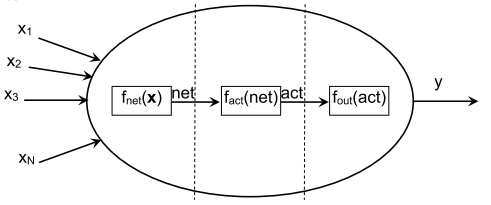
\includegraphics[width=0.5\linewidth]{Figures/artificial_neuron.png}
    \caption{Three stage model of an artificial neuron \cite{Bartz2018}.}
    \label{fig:artifical_neuron}
\end{figure}
\newline
In the first stage, the input stimuli of the neuron are combined into a so-called net-value. This net-value leads to a particular level of activity within the neuron. Although, for some classification tasks there are also other possibilities like distance from center \cite{Schwenker2001}, most times a weighted sum is used as a net function. In the definition of net sometimes a base level of excitation is stated, which is taken into account by a so-called bias value $\Theta$. To allow a compact notation this bias value is usually given as a fixed input value $x_0 = -1$ and a corresponding weight, so that $\Theta = -w_0$. The weighted sum can then be notated as:
\begin{equation}
    \label{eq:net}
    net = \sum_{n=0}^N\omega_n \cdot x_n
\end{equation}
After multiple inputs are combined into a cumulative net value the next stage is the so-called activation function $f_{act}$. This function is normally a monotonously increasing function of net. Figure @todo shows some popular examples.

The third and last stage is the output function, which imitates the effects of the axon and the synaptic connection. This stage is very often neglected because the goal of the model is not to copy the biological behavior as accurately as possible but to provide a processing tool inspired by neural mechanisms. So the output value in most cases is the same as the activation value, it holds $y = act$. In this case, the output function is an identity function (see fig. @todo).
\subsection{Multi Layer Perceptron}
The most commonly used form of artificial neural networks is the form of a multi layer perceptron. The perceptron is the fundamental unit in deep learning models. It can perform a basic mathematical operation, more specifically it can linearly
combine a set of incoming values from it's inputs. The MLP features multiple layers of perceptrons, where each neuron is connected to all neurons of the following layer, forming a fully connected network.
\section{Deep Learning}
Deep learning describes a set of machine learning methods for ANNs with multiple hidden layers. One can classify the learning methods of ANNs into three basic categories:  supervised learning, unsupervised learning, and reinforcement learning. Although this work concentrates on reinforcement learning, we will have a short look at the other two methods.
\subsection{Supervised Learning}
As the term supervised learning suggests, human supervision is necessary for the ANN to learn. In most cases, this means, that the training data has been labeled with human insight beforehand so that the samples contain both input and desired output values. During the learning process, the calculated output of the ANN is compared to the correctly labeled output of the sample, and an error or divergence is measured. This error is then used to adjust the connecting weights within the network. This way the network can achieve better performance and minimize the error in the next epoch of training. 
Training is considered successful, if the resulting error lies within an acceptable range, for all samples of the training dataset.
As of today, the most used algorithm for supervised learning is Back-propagation, implemented successfully by Rumelhart in 1985 \cite{Rumelhart1985}\cite{Patterson1997}.
\subsection{Unsupervised Learning}
Machine learning without known target values or rewards granted by the environment is generally defined as unsupervised learning. The learner tries to recognize patterns and statistical regularities that stand out from the amorphous noise. During training, the learner machine intensifies specific connection weights so that the results for the clustering of central, representative datasets match up \cite{Patterson1997}. Popular fields of use are automated clustering of data points or compressing data to achieve dimensional reduction.
\section{Deep Reinforcement Learning}
Machine learning as a field of science has been around for decades now. It is part of the overall field of artificial intelligence and enables systems to recognize patterns and regularities on the basis of datasets.
One could say knowledge is derived from experiences. So in Reinforcement Learning, like a human, the AI agent learns from the consequences of its actions, rather than being explicitly taught. This feedback loop is what reinforcement learning is about.
And it is on the rise. Most outstanding achievements in deep learning were made due to deep reinforcement learning. DeepMind's AI agents teach themselves how to walk, run and overcome obstacles.
Google's Alpha Go has beaten the world's best human player in the board game Go, Google's Alpha Star is reaching high levels of play in the
video game StarCraft II, the game which will be used for experiments in this project as well.
\newline
\begin{figure}
    \centering
    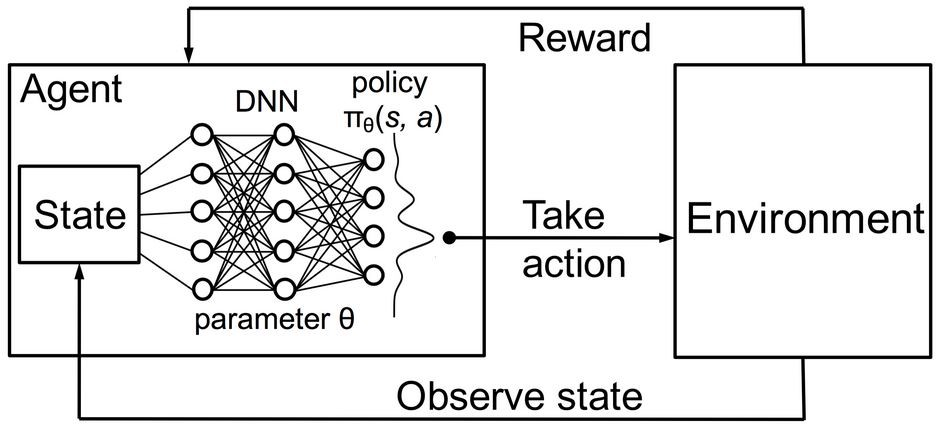
\includegraphics[width={0.5\linewidth}]{Figures/DRL_schemantic_depiction.jpeg}
    \caption{Schematic depiction of a reinforcement learning process.}
    \label{fig:drl_schemantic}
\end{figure}
In Deep Reinforcement Learning, the Agent is represented by a neural network, which stores a representation of the experiences made in its environment. The agent observes the current state of the environment and decides which action to take from a pool of actions, called the action space.
The decision is made on the basis of the current state and past experiences. Based on the taken action, the environment occasionally provides the agent with a reward. The amount of reward determines the quality of the taken action with regards to solving the given problem.
The objective of an AI agent is to maximize the accumulated reward over time, by learning to take the right actions in any given circumstances.
However, the reward is mostly delayed, thus not instantaneous. This makes time play a fundamental role in reinforcement learning and the decision process it revolves around.
This decision process can be modeled as a Markov Decision Process, laying the cornerstone for modern reinforcement learning algorithms which are described in the following sections.
\subsection{Markov Decision Process}
A Markov Decision Process (MDP) is a discrete time stochastic control process. MDP is the state of the art approach to model the complex environment of an AI agent. An MDP is defined by the tuple ${\{S, A, P, R, \gamma\}}$. A and S are finite sets of actions and states. P is a state transition probability matrix. R is the reward expected by the agent. In the following the MDP will be build up step by step. \newline
Every problem that the agent is supposed to solve can be considered as a sequence of states (a state may be for example a chess board configuration). While taking actions, the agent moves from one state to another. In a Markov Process, the current state depends only on the previous state. This is also called the Markov Property (\ref{eq:markov_prop}).
\begin{equation}
    \label{eq:markov_prop}
    P[S_{t+1}|S_t] = P[S_{t+1}|S_1,S_2,S_3,...,S_t]
\end{equation}
A Markov Process is a memoryless random process. It is a sequence of random states, with each state fulfilling the Markov property. This means that the probability distribution of the next state is fully determined by just the current state and not any other state. A transition happens with a certain probability ${Pss'}$
\begin{equation}
    \label{eq:trans_prob}
    Pss' = P[S_{t+1} = s' | S_t =s]
\end{equation}
The state transition matrix ${P}$ defines transition probabilities from all states $s$ to all successor states ${s'}$:
\begin{equation}
    \label{eq:trans_matrix}
    P = \begin{bmatrix}
        P_{11} & \dots & P_{1n}\\
        \vdots & \ddots & \vdots\\
        P_{n1} & \dots & P_{nn}\\
    \end{bmatrix}
\end{equation}
Now, in reinforcement learning, we add a reward function ${R}$ to the process.  ${R}$ defines the reward that the agent will receive at the next time step when being in state $s$ at time $t$:
\begin{equation}
    \label{eq:reward_func}
    R_s = \mathbb{E}[R_{t+1}|S_t = s]
\end{equation}
This way we get a Markov chain with values called a Markov Reward Process.
Since the Markov Process is a stochastic process, the reward given by the value function has to be seen as an expected reward.
 Reward, sticking to the chess game example, means certain states of the board are more promising than others in terms of the potential to win the game. After all, the total reward $G_t$(\ref{eq:markov_reward}), which is the expected accumulated reward across the sequence of all states.
\begin{equation}
    \label{eq:markov_reward}
    G_t = R_{t+1} + R_{t+2} + ... = \sum_{k=0}^\infty R_{t+k+1}
\end{equation}
 Every reward is weighted by the so-called discount factor $\gamma \in [0, 1]$, shown in \ref{eq:disc_markov_reward}.
 \begin{equation}
    \label{eq:disc_markov_reward}
    G_t = R_{t+1} + \gamma R_{t+2} + ... = \sum_{k=0}^\infty \gamma^kR_{t+k+1}
 \end{equation}
 The higher the factor, the less important are rewards that lie further into the future. This is beneficial, since immediate rewards may earn more interest than delayed and hence more uncertain rewards. Conveniently, it also helps to eliminate infinite returns in a cyclic Markov process.
These value of a state is defined by the value function ${v(s)}$, which gives the long-term value of a state $s$. Or in other words, it determines the amount of reward the agent can get starting in state $s$ until the process terminates:
\begin{equation}
    \label{eq:value_func}
    v(s) = \mathbb{E}[G_t|S_t =s]
\end{equation}
The value function can be decomposed into two parts: Immediate reward $R_{t+1}$ and the discounted value of successor state ${\gamma v(S_{t+1})}$. This way, one can concisely express the so-called Bellman equation using matrices and the column vector $v$, containing one entry per state from 1 to $n$:
\begin{equation*}
    v = R + \gamma Pv
\end{equation*}
\begin{equation}
    \label{eq:bellman_matrix}
    \begin{bmatrix}
        v(1)\\
        \vdots\\
        v(n)\\
    \end{bmatrix} = \begin{bmatrix}
        R_1\\
        \vdots\\
        R_n\\
    \end{bmatrix} + \gamma \begin{bmatrix}
        P_{11} & \dots & P_{1n}\\
        \vdots\\
        P_{n1} & \dots & P_{nn}\\
    \end{bmatrix}  
    \begin{bmatrix}
        v(1)\\
        \vdots\\
        v(n)\\
    \end{bmatrix}
\end{equation}
The Bellman equation (\ref{eq:bellman_matrix}) can be solved directly as it is a linear equation. However, as the complexity of the underlying Markov process increases, the problem becomes too big to be solved directly as the computational complexity for the Bellman equation is $O(n^3)$ for $n$ states.
\newline
Now in an MDP, the next state is not only dependent on the current state, but also on the action the agent takes in that state. Therefore, the taken action $a$ has to be added to (\ref{eq:trans_prob}) and (\ref{eq:reward_func}):
\begin{equation}
    \label{eq:trans_prob_with_action}
    P_{ss'}^a = P[S_{t+1} = s' | S_t =s, A_t = a]
\end{equation}
\begin{equation}
    \label{eq:reward_func_with_action}
    R_s^a = \mathbb{E}[R_{t+1}|S_t = s, A_t = a]
\end{equation}
The MDP describes the basis for an algorithm popularly used for reinforcement learning, called Q-Learning, which the next section will cover.
\subsection{Q-Learning and DQN}\label{sec:q-learning}
Q-learning is an off-policy TD control algorithm that seeks to find the best action to take given the current state. It was invented by Christopher Watkins in 1989 and is defined by:
\begin{equation}
    \label{eq:q_learn}
    Q(S_t, A_t) \leftarrow Q(S_t, A_t) + \alpha [R_{t+1}+\gamma \max_aQ(S_{t+1},a)-Q(S_t,A_t)]
\end{equation}
It is considered off-policy because the q-learning function learns from actions that are outside the current policy, like taking random actions. More specifically, q-learning seeks to learn a policy that maximizes the total reward. It is making use of a model-free prediction and control methods.

In this case, the learned action-value function, Q, directly approximates q, the optimal
action-value function, independent of the policy being followed. The Q-value resembles the discounted value of a state-action pair. This dramatically
simplifies the analysis of the algorithm and enabled early convergence proofs. The policy however
still affects control because it determines which state-action pairs are visited and updated.
However, all that is required for correct convergence is that all pairs continue to be
updated. This is a minimal requirement in the sense that
any method guaranteed to find optimal behavior in the general case must require it.
Under this assumption and a variant of the usual stochastic approximation conditions on
the sequence of step-size parameters, Q has been shown to converge with probability 1 to
q. The Q-learning algorithm is shown below in the procedural form\cite{Sutton2015}:
\begin{algorithm}
    \caption{Q-learning for estimating a policy $\pi$}
    \begin{algorithmic}
    \State Algorithm parameters: step size $\alpha \in (0, 1]$, small  $\epsilon > 0$
    \State Initialize $Q(s,a)$, for all $s\in S^+$, $a\in A(s)$, arbitrarily except that $Q(terminal)=0$
    \State Loop for each episode:
    \While{$S$ is not terminal}
        \State Initialize $S$
        \ForAll{step of episode}
            \State Choose $A$ from $S$ using policy derived from $Q$ (e.g., $\epsilon$-greedy)
            \State Take action $A$, observe $R$, $S'$
            \State $Q(S, A) \leftarrow Q(S, A) + \alpha [R'+\gamma \max_aQ(S',a)-Q(S,A)]$
            \State $S \leftarrow S'$
        \EndFor
    \EndWhile
    \end{algorithmic}
\end{algorithm}

The following figure (\ref{fig:dql_procedure}) is a depiction of the Q-learning process for DQNs, using an online and a target network. It shows how the online DQN, given the current state $S_t$, predicts the values of actions. Then it selects the best action based on an $\epsilon$ greedy policy and observes the environment's reaction to the action taken. In the {\it collect experience} block, all observations from the environment are collected. Like the received rewards and the state, the agent ends up in.

\begin{figure}
    \centering
    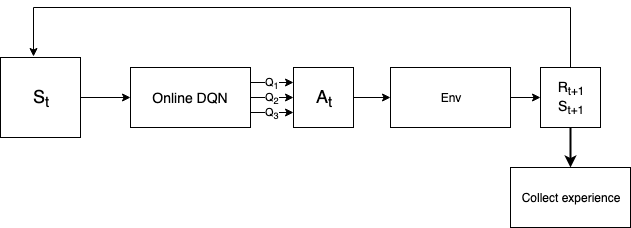
\includegraphics[width=0.8\linewidth]{Figures/QLearningProcedure.png}
    \caption{Deep Q-learning Procedure}
    \label{fig:dql_procedure}
\end{figure}
Once enough experience has been collected, one can start training the online neural network while keeping the target network fixed. After a set amount of steps, the weights of the two networks get synchronized. Minh et al \cite{Mnih2016} suggest selecting so-called mini-batches of size 32 from the pool of collected experiences for training. The following equation \ref{eq:exp_tuple} describes an experience tuple. It contains state, action, immediate reward, and the following state:

\begin{equation}
    \label{eq:exp_tuple}
    e_t = (s_t, a_t, r_{t+1}, s_{t+1})
\end{equation}

Equation \ref{eq:target_q_value} shows how the target Q-value can be calculated. From the experience, we already know the immediate reward $R_{t+1}$. Gamma ($\gamma$) is the discounting factor which is multiplied by the argmax of the Q-values predicted by the target DQN. In other words, the action with the highest predicted Q-value gets selected and discounted for the target Q-value.

\begin{equation}
    \label{eq:target_q_value}
    Y_t^{DQN} = R_{t+1} + \gamma \cdot max_aQ'(a)
\end{equation}

One thing to note here is that at this stage we are using an untrained target DQN to predict the future rewards and select the maximum of its predictions. This is introducing a strong bias towards that maximum, a weakness of the Q-learning algorithm that is discussed in \ref{sec:double_q_learning}. 

Having calculated the target Q-value, one can subtract the predicted Q-value for the action taken and thereby calculate the loss, see equation \ref{eq:loss_function}.
\begin{equation}
    \label{eq:loss_function}
    Loss = [Y_t^{DQN} - Q(A_t)]^2
\end{equation}
This method resembles a stochastic gradient descent, updating the current value $Q$ towards the target $Y_t^{DQM}$ one can now update the weights in the online DQN and repeat the process.

As proven by Hasselt, Guez, and Silver \cite{VanHasselt2015}, the Q-learning algorithm suffers from its argmax component overestimating action values. Thus, they introduced the Double Q-Learning method, which will be covered in the next section.

\subsection{Double-Q-Learning}\label{sec:double_q_learning}
In standard Q-Learning and DQN, as seen in \ref{sec:q-learning}, the max operator uses the same values both to select and evaluate an action. This makes it more likely to select overestimated values, resulting in overoptimistic value estimates, because the network might be making a false prediction and then evaluates this prediction with the same values. To prevent this, (van Hasselt, 2010) introduced the idea to decouple the selection from the evaluation. This method is called {\it Double Q-learning}. In the original Double Q-learning algorithm, two value functions are learned by assigning each experience randomly to update one of the two value functions, such that there are two sets of weights. For each update, one set of weights is used to determine the greedy policy and the other to determine its value. As \cite{VanHasselt2015} show, we can untangle the selection and evaluation of actions in Q-learning by rewriting its target (\ref{eq:target_q_value}) as

\begin{equation}
    \label{eq:q_target_untangled}
    Y_t^Q = R_{t+1} + \gamma \cdot Q(S_{t+1}, max_a Q(S_{t+1}, a;  \theta_t); \theta_t).
\end{equation}
Followed by the Double Q-learning Error, showing that the selection of the action still uses the weight set $\theta_t$ of the online DQN. The evaluation however happens based on the second set of weights $\theta'_t$: 
\begin{equation}
    \label{eq:double_q_target}
    Y_t^Q = R_{t+1} + \gamma \cdot Q(S_{t+1}, max_a Q(S_{t+1}, a;  \theta_t); \theta'_t).
\end{equation}
The procedure for the Double Q-Learning algorithm can be described as follows:
\begin{algorithm}
    \caption{Double Q-learning}
    \begin{algorithmic}
    \State Algorithm parameters: step size $\alpha \in (0, 1]$, small  $\epsilon > 0$
    \State Initialize $Q(s,a)$, for all $s\in S^+$, $a\in A(s)$, arbitrarily except that $Q(terminal)=0$
    \State Initialize $c$, set $\tau$
    \State Loop for each episode:
    \While{$S$ is not terminal}
        \State Initialize $S$
        \State $c += 1$
        \ForAll{step of episode}
            \State Choose $A$ from $S$ using policy derived from $Q$ (e.g., $\epsilon$-greedy)
            \State Take action $A$, observe $R$, $S'$
            \State $Q(S, A) \leftarrow Q(S, A) + \alpha [R_{t+1}+\gamma \cdot Q(S_{t+1}, max_a Q(S_{t+1}, a;  \theta_t); \theta'_t)]$
            \State $S \leftarrow S'$
            \State $\theta_t \leftrightarrow \theta'_t$ (switch roles of weight sets)
        \EndFor
        \If{$c >= \tau$}
            \State $\theta_target = \theta_t $ (synchronize weights of target network)
            \State $c = 0$
        \EndIf
    \EndWhile
    \end{algorithmic}
\end{algorithm}
\newpage
In their empirical results, see \cite{VanHasselt2015}, van Hasselt et al. describe that the Double DQN improves over DQN both in terms of value accuracy and in terms of policy quality. They state that, in their tests the Double DQN produces more accurate value estimates and also better polices, by successfully reducing standard DQN's overestimations.
\subsection{Distributed Prioritized Experience Replay}
Online reinforcement learning agents using simple algorithms, like the standard q-learning, are prone to miss potentially important experiences. This is because they incrementally update their policy or value function parameters while they observe a stream of experience. Although they actually observe the experience, due to immediate discarding the possibly rare experience is forgotten quite rapidly.
{\it Experience replay}, see \cite{Lin2014}, successfully addresses this issue by storing experience in a replay memory. With the help of this memory, we can update the parameters also based on rarely occurring experiences by using them more than once. The DQN implements this technique to stabilize the training of a deep neural network. By using a large sliding window replay memory this results in effectively processing each experience tuple eight times, see \cite{Schaul2016} and section \ref{sec:q-learning}.
{\it Prioritized Experience Replay}, see \cite{Schaul2016}, makes enhancements by introducing prioritization on which experiences in memory are replayed to make experience replay more efficient and effective. As stated by \cite{Schmidhuber1991CuriousMC}, it is hard to determine whether or not an experience is more task-relevant than others. Some might also become more useful as the agent's competence to solve the task at hand increases. Prioritized replay liberates agents from considering experiences with the same frequency that they are experienced, however introducing some bias and loss of diversity, see \cite{Schaul2016}.
To overcome the issue of losing diversity, a stochastic sampling method defines the probability of sampling experience $i$ as
\begin{equation*}
    P(i) = \frac{p_i^\alpha}{\sum{_k p_k^\alpha}}
\end{equation*}
where $p_i > 0$ is the priority of the experience $i$ in memory. The exponent $\alpha$ determines how much prioritization is used, with $\alpha = 0$ corresponding to the uniform case \cite{Schaul2016}.
When estimating the expected value through stochastic updates, the updates have to correspond to the same distribution as its expectation. Otherwise, the solution that the learning algorithm will converge to will be changed. If not corrected, prioritized replay changes this distribution in an uncontrolled fashion. The bias can be corrected by using importance-sampling (IS) weights to compensate for the non-uniform probabilities $P(i)$ if $\beta = 1$. See the usage of $w_i\delta_i$ instead of $\delta_i$ in Algorithm \ref{alg:prioritizedReplay}. $\beta$ is linearly increased during learning, meaning that compensation is best towards the end of the process. Tom Schaul et al. at GoogleDeepMind hypothesize, that a small bias, in the beginning, can be ignored because the process is highly non-stationary anyway at that time.
\begin{equation}
    P(i) = \frac{p_i^\alpha}{\sum{_k p_k^\alpha}}
\end{equation}
where $p_i > 0$ is the priority of the experience $i$ in memory. The exponent $\alpha$ determines how much prioritization is used, with $\alpha = 0$ corresponding to the uniform case \cite{Schaul2016}.
\begin{algorithm}
    \label{alg:prioritizedReplay}
    \caption{Double DQN with proportional prioritization \cite{Schaul2016}}
    \begin{algorithmic}
    \State Input: mini-batch $k$, step-size $\eta$, replay period $K$ and size $N$, exponents $\alpha$ and $\beta$, budget $T$.
    \State Initialize replay memory $H = \varnothing, \Delta = 0, p1 = 1$
    \State Observe $S_0$ and choose $A_0 \sim \pi_\theta(S_0)$
    \For{t=1 {\bf to} $T$}
        \State Observe $S_t$, $R_t$, $\gamma_t$
        \State Store experience tuple ($S_{t-1,} A_{t-1}, R_t, \gamma_t, S_t$) in $H$ with maximal priority $p_t = max_{i<t}p_i$
        \If{$t \equiv 0$ mod $K$}
            \For{j=1 {\bf to} $k$}
                \State Sample experience $j ~ P(j) = p^\alpha_j/\sum_i{p^\alpha_i}$
                \State Compute importance-sampling weight $w_j = / N \cdot P(j))^{-\beta}$
                \State Compute TD-error $\delta_j = R_j + \gamma_jQ_{target}(S_j, max_aQ(S_j,a)) - Q(S_{j-1},A_{j-1})$
                \State Update experience priority $p_j \leftarrow |\delta_j|$
                \State Accumulate weight-change $\Delta \leftarrow \Delta + w_j \cdot \delta_j \cdot \nabla_\Theta Q(S_{j-1}, A_{j-1})$
            \EndFor
            \State Update weights $\Theta \leftarrow \Theta + \eta \cdot \Delta, reset \Delta = 0$
            \State From time to time copy weights into target network $\theta_{target} \leftarrow \theta$
        \EndIf
        \State Choose action $A_t \sim \pi_\theta(S_t)$
    \EndFor
    \end{algorithmic}
\end{algorithm}

\section{StarCraft II}\label{sec:SC2}
The testbed game used for this research project is Blizzard Entertainment's StarCraft II, released worldwide in July 2010 for Microsoft Windows and Mac OS X. StarCraft II is a science fiction real-time strategy video game and the sequel to the 1998 video game StarCraft. Since 2017, StarCraft II is free-to-play. The game is played professionally throughout the world. Just like its predecessor StarCraft: Brood War, the highest level of play is centered in South Korea. During its early years, it was considered the largest esport in the world.
When choosing a game to use as an environment and testbed to train reinforcement agents in, StarCraft II is especially suited for this purpose, as Blizzard Entertainment provides a communication interface and protocol for interacting with the game client (see section \ref{sec:SC2API}).
The game focuses on three different races: Terran, Zerg, and Protoss. Each race has different units and tactics. The strengths and weaknesses of the races allow many different strategies.
To build structures or units for combat, you need two resources: minerals and vespin gas, where minerals are always needed, vespin gas only for more advanced buildings and troops. Minerals can be mined from mineral fields, while vespin gas can be extracted from vespin geysers, for which special buildings must be placed on the geysers. The number of mineral fields and vespin geysers varies per map, so there are more mineral fields and vespin geysers on a 4v4 map than on a 1v1 map.
In competitive setups, one starts with eight mineral fields and two vespin geysers. As the game progresses, however, one should mine and expand more mineral and vespin gas storage sites to build more and better units and buildings. This expansion has to be considered as well as warfare with the enemy party.
The key to victory is often having the more powerful units at the right place and at the right time in order to beat the opponent's forces.
However, units cannot be built arbitrarily, as most units have a certain building as a prerequisite. The right tactics and the strategic use of these units form the framework for a successful battle. For example, some units can only attack air or ground units. Some units can camouflage themselves and can only be detected with detector units. In addition, each unit type has a number of attributes that make it particularly effective or vulnerable in certain scenarios. Thus, a perfect army composition is essential, taking into account the constellation of your opponent. There are countless possibilities for combinations and successful tactics, whereby the terrain can also be included. For example, units with an elevated position have a visual advantage.
While the main objective of the game is to beat the opponent, the player must also carry out and manage a number of sub-tasks, such as gathering resources or building structures. Games can last anywhere from a few minutes to one hour to complete, meaning actions taken early in the game might first pay-off in the long run. Finally, the map or the games state is only partially observed, meaning agents must use a combination of memory and planning to succeed.
StarCraft II updates the simulation 22.4 times per second. The game is mostly deterministic, but it does have some randomness mainly for cosmetic reasons, like weapon speed (fire rate) and update order. This randomness, however, can be negated by the use of a random seed \cite{DBLP:journals/corr/abs-1708-04782}.
The next section describes, how we used StarCraft II and a set of tools to implement different reinforcement learning algorithms.
\section{Implementation}
Applied reinforcement learning can require the use of multiple complex systems to cope with the needs of of training, simulation, and serving steps. In this section the software systems used in this work will be covered. Starting with the framework for serving the training process.
\subsection{Ray Framework}
Ray is a framework for building and running distributed applications, developed at the Berkeley University of California especially for AI applications. As agents of modern reinforcement learning systems will have to continuously interact with the environment and learn from these interactions, they impose demanding system requirements, see \cite{Moritz2017}. Ray implements a unified interface that can ship both task-parallel and actor-based computations in a single execution engine.
It features a distributed scheduler and a distributed and fault-tolerant store to manage the system's control state.
For dealing with large reinforcement learning workloads, Ray implements the evolutions strategies algorithm. The algorithm broadcasts a new policy to a pool of workers and aggregates the results of around 10000 tasks, where each performs 10 to 1000 simulation steps, see \cite{Moritz2017}.
In this project, the Ray system is used to have 10 simultaneous StarCraft II matches played out in highly increased game speed by agents fed from one online DQN.
The Ray framework also supplies a library especially crafted for reinforcement learning. It features top-down hierarchical control for the many short-running computation tasks occurring during distributed reinforcement learning tasks. The benefits are described in the next section.
\subsection{RLlib}
Since modern reinforcement learning algorithms are highly irregular in the computation patterns they create, it is highly useful to have a system at hand that makes the implementation of different algorithms easy. As we want to compare the performance of different algorithms learning to play StarCraft II, we decided to use RLlib. It centralizes program control, instead of having to manage each process on its own, making parallelization very convenient. As shown in Figure \ref{fig:DRL_control_model}, a single {\it driver program} can delegate the algorithm sub-tasks to other processes, enabling parallel execution. $A$, $B$, and $C$ still hold their state, like their active policy or their general simulation state, but wait passively until called by $D$.  Furthermore, through RLlib's hierarchical delegation of control, the worker processes $B$ and $C$ can further delegate work, like gradient computation, to sub-workers of their own when executing tasks \cite{Liang2017}.
The way the implementation works with RLlib is as follows. First, we specify a policy model $\pi$, which maps current observation $o_t$  to an action $a_t$ and the next RNN state $h_{t+1}$. As an option, the current hidden state $h_t$ can also be stored.
\begin{equation}
    \label{eq:policy_graph}
    \pi_\theta(o_t, h_t) \Rightarrow (a_t,h_{t+1}, y_t^1 ... y_t^N)
\end{equation}

Like shown in \ref{sec:q-learning}, gradient-based algorithms define a combined loss $L$ that can be descended to improve the policy and possible auxiliary networks:
\begin{equation}
    \label{eq:combined_loss}
    L(\theta; X) \Rightarrow loss
\end{equation}

\begin{figure}
    \centering
    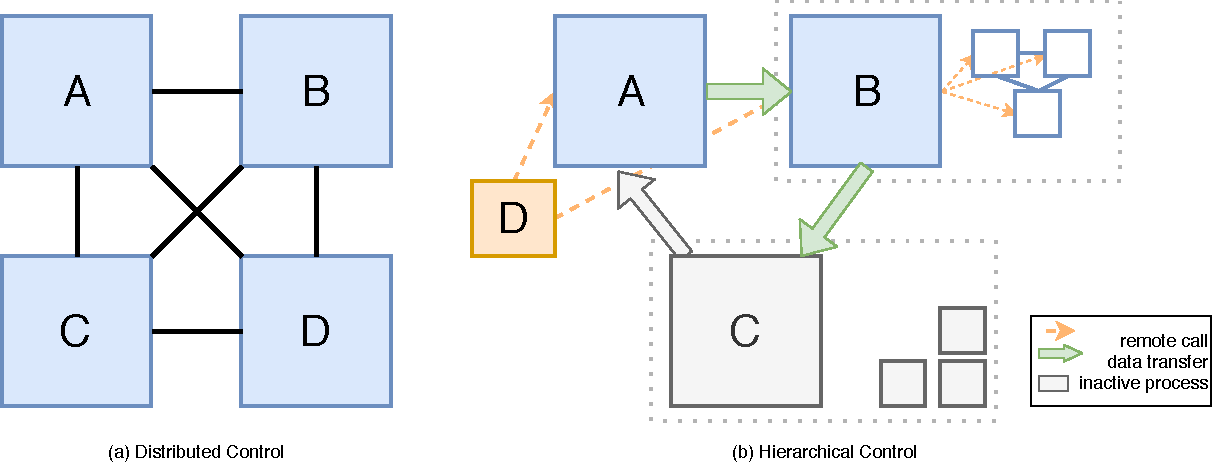
\includegraphics[width=\linewidth]{Figures/DRL_Control_Model.pdf}
    \caption{RLlib component control \cite{Liang2017}}
    \label{fig:DRL_control_model}
\end{figure}
\subsection{Policy Optimization}
Using RLlib, we can separate the implementation of algorithms, which are defined in the declaration of the policy graph, and the choice of an algorithm-specific {\it policy optimizer}. This policy optimizer will perform distributed sampling, parameter updates and manage the replay buffers. To distribute the computation, the optimizer operates over a set of policy evaluator replicas. This separation enables the reinforcement learning task to make better use of available resources or algorithm features, see \cite{Liang2017}.

\subsection{DQN implementation}
As a first implementation of a reinforcement learning algorithm we used the architecture presented by Minh et al. in 2015 \cite{Mnih2016}, known as DQN, see also section \ref{sec:q-learning}. The DQN architecture may have been outperformed by the more recent algorithms, however, it can still act as a baseline experiment for our optimization scenario. RLlib DQN is implemented using the {\it SyncReplayOptimizer}, a policy optimizer provided by Ray. The algorithm can optionally be scaled effectively by increasing the number of workers collecting samples in parallel, however, by default this is set to one worker. See table \ref{tab:dqn_params} for the set of parameters used in the DQN implementation. Parameter numbers one to three affect the model, four to nine the optimization and ten to 14 the exploration behavior. We use an $\epsilon greedy$ policy with exploration annealing from $\epsilon_{start} = 1.0$ to $\epsilon_{final} = 0.02$ by the scaling fraction $0.1$. This means the final value of random action probability equals $0.02$. 
\begin{table}
    \begin{center}
        \begin{tabular}{| c | c | c |}
            \hline
            Nr. & {\bf Parameter} & {\bf Value} \\
            \hline
            \hline
            1 & N-step Q learning & 1 \\
            \hline
            2 & Hidden layers & [256,256,256,256] \\
            \hline
            3 & Number of parallel workers & 1 \\
            \hline
            \hline
            4 & Learning rate & 5e-4 \\
            \hline
            5 &Adam $\epsilon$ & 1e-8 \\
            \hline
            6 & Gradient clipping at & 40 \\
            \hline
            7 & Sample batch size & 4 \\
            \hline
            8 & Train batch size & 32 \\
            \hline
            9 & Noisy network & false \\
            \hline
            \hline
            10 & Exploration $\epsilon_{start}$ & 1.0 \\
            \hline
            11 & Exploration $\epsilon$ fraction & 0.1 \\
            \hline
            12 & Exploration $\epsilon$ num time-steps & 100000 \\
            \hline
            13 & Exploration $\epsilon_{final}$ & 0.02 \\
            \hline
            14 & Target network update frequency $\tau$ & 500 \\
            \hline
        \end{tabular}
        \caption{Parameter set used for DQN in RLlib}
        \label{tab:dqn_params}
    \end{center}
\end{table} 
\subsection{Ape-X implementation}
For the distributed prioritized experience replay, commonly referred to as Ape-X, we use RLlib's provided Ape-X implementation.
We can describe the Ape-X architecture as follows; multiple actors, each with its own instance of the environment,
generate experience, add it to a shared experience replay memory, and compute initial priorities for the data.
The (single) learner samples from this memory and updates the network and the priorities of the experience in
the memory. The actors’ networks are periodically updated with the latest network parameters from the learner. Figure \ref{fig:apexnutshell} depicts the architecture. As you can see, all actor agents share one common replay memory, as opposed to the Double-DQN, where each actor writes experiences to it's own replay memory.
\begin{figure}
    \centering
    \includegraphics[width=\linewidth]{Figures/apexnutshell.png}
    \caption{The Ape-X architecture \cite{DBLP:journals/corr/abs-1803-00933}}
    \label{fig:apexnutshell}
\end{figure}
For the set of parameters used for Ape-X, please refer to table \ref{tab:apex_params}.
\begin{table}
    \begin{center}
        \begin{tabular}{| c | c | c | c |}
            \hline
            Nr. & {\bf Parameter} & {\bf Symbol} & {\bf Value} \\
            \hline
            \hline
            1 & N-step Q learning &  & 1 \\
            \hline
            2 & Hidden layers &  & [256,256,256,256] \\
            \hline
            3 & Number of parallel workers &  & 1 \\
            \hline
            \hline
            4 & Learning rate & $\eta$ & $5 \cdot 10^4$ \\
            \hline
            5 & Discount factor & $\gamma$ & 0.99 \\
            \hline
            6 &Adam epsilon & $\epsilon_{Adam}$ & $1 \cdot 10^{-8}$ \\
            \hline
            7 & Gradient clipping at &  & 40 \\
            \hline
            8 & Sample batch size & & 4 \\
            \hline
            9 & Train batch size &  & 32 \\
            \hline
            10 & Noisy network &  & false \\
            \hline
            \hline
            11 & Exploration initial & $\epsilon_{start}$ & 1.0 \\
            \hline
            12 & Exploration fraction & $\epsilon_{frac}$ & 0.1 \\
            \hline
            13 & Exploration num time-steps &  & 100000 \\
            \hline
            14 & Exploration final & $\epsilon_{final}$ & 0.02 \\
            \hline
            15 & Target network update frequency & $\tau$ & 500 \\
            \hline
        \end{tabular}
        \caption{Parameter set used for Ape-X in RLlib}
        \label{tab:apex_params}
    \end{center}
\end{table} 
\subsection{StarCraft II Learning Environment}
One of the main reasons for choosing StarCraft II, see section \ref{sec:SC2}, as our testbed game is the release of the StarCraft II Learning Environment (SC2LE). It is a set of tools that is aimed towards the needs of researchers of AI in real-time strategy games. It includes the StarCraft II Machine Learning API developed by Blizzard Entertainment, providing developers and researchers hooks into the game, making the observation of the game state much easier and convenient. Along with that an open-source version of DeepMind's toolset, PySC2 and a dataset of anonymized game replays. The following section describes how we used SC2LE API and the PySC2 toolset to create a feature vector for our agent.
\label{sec:SC2API}
\subsubsection{StarCraft II Machine Learning API}
When we want to have our agents interact with StarCraft, we must implement some sort of interface for the online policy network to receive the game's state and deliver picked agents to the StarCraft client. In this case we used the SC2LE API and the wrapper libraries PySC2 and PythonSC2 to extract a set of picked values to supply our agent with information we decided to be useful for our defined optimization scenario, see section \ref{sec:scenario}. For an overview of these picked values see the following section. In section \ref{sec:action} is described, what discrete actions we prepared for the learning agents, using the PythonSC2 library.
\subsubsection{Observed State}
The agent perceives its environment through observation after every action taken. The observation of the SC2LE game state happens with the help of a custom build feature vector. The PySC2 toolset provides nearly every information the game client holds, however not all of these features are necessary for the learning goal. In an attempt to simplify the reinforcement learning problem we picked features directly related to the task given and thus, we proclaim, the most relevant ones, see table \ref{tab:observation}.
\begin{table}
    \begin{center}
        \begin{tabular}{ | c | c || c | }
            \hline
            {\bf Feature} & {\bf Content} & {\bf Value-Range} \\
            \hline
            1 & minerals & -500 to 30000\\ 
            \hline
            2 & supply\_left & 0 to 200 \\  
            \hline
            3 & supply\_used & 0 to 200 \\
            \hline
            4 & frame & 0 to 20000 \\
            \hline
            5 & supply Depots & 0 to 200 \\
            \hline
            6 & barracks & 0 to 200 \\
            \hline
            7 & workers & 0 to 200 \\
            \hline
            7 & marines & 0 to 200 \\
            \hline
        \end{tabular}
    \end{center}
    \caption{Observation feature vector}
    \label{tab:observation}
\end{table}

$Minerals$, are the only resource needed for the task Their range starts at negative 500 because sometimes the policy server would crash due to a negative amount in this feature. We assume this is a bug in the SC2LE. $supply\_left$ is a critical feature as it indicates when building another supply depot building is required. Each supply depot provides 10 additional supplies. $frame$ is the number of in-game frames that have been processed since the start of the game. This gives somewhat of a time estimation as the game runs at 24 frames per second. Features 5 to 8 show the number of the respective unit or building.
\subsubsection{Action Space}\label{sec:action}
StarCraft's action space presents a challenge with a choice of more than 300 basic actions that can be taken. Contrast this with the Atari games, which only have about ten, most times less than that. On top of this, actions in StarCraft are hierarchical and can sometimes be modified or augmented.
In an effort to reduce problem complexity and provide the algorithms with discrete actions to choose from, we decided on four different scripted action paths plus the ability to do nothing. The pool of possible actions to choose from at any state of our testbed scenario is presented in table \ref{tab:actions}. At first, it was planned to be expanded later on, but after a number of experiments with the limited action space, we decided that enlargement of possible actions would not be beneficial to the project, see section \ref{sec:results}.
\begin{table}
    \begin{center}
        \begin{tabular}{ c | c | c }
            {\bf Action} & {\bf Effect} & {\bf Prerequisites} \\
            \hline
            build\_worker & Produces worker unit to increase mineral income. & None \\ 
            build\_marine & Produce marine unit. Provides reward. & Barracks \\  
            build\_supply & Build supply depot. Provides supply. & Worker \\
            build\_barracks & Build barracks. Can produce marines. & Supply Depot \\
            no\_action & Do nothing. & None    
        \end{tabular}
    \end{center}
    \caption{The agents action space}
    \label{tab:actions}
\end{table}

\section{Experiment}
In this chapter the experiments made in context of this project will be presented. Experiments have been carried out throughout, while making changes to the underlying implementation. This means not all results are directly comparable. Therefore, the most useful results will be evaluated and their possible shortcomings will be discussed.
\subsection{Optimization Scenario}\label{sec:scenario}
Since StarCraft II's standard game features a very complex and very demanding environment for our reinforcement learning agents we had to reduce the problem complexity.
A game of StarCraft II is mostly about having more strike force at the right time and the right place than the opponent.
So one of the most important tasks when learning the game is the ability to produce as many armed forces as fast as possible. Following that idea, we picked an optimization scenario that reflects that problem in the simplest way provided by the game.
In the scope of this work, we focus on the Terran race, so the most straight forward approach is to produce marines from the barracks building.
Therefore, as a first experiment for the reinforcement learning agent, a scenario is used, where it's the goal is solely to train marines.
The agent receives a reward for every marine trained in a game of six minutes of game time. The time limit is picked on purpose because in a real match this would be the point where a mass of marines would be the most useful.
In order to reach the optimal amount of marines in the given time frame, the agent must optimize its use of resources.
As a benchmark, we @TODO(check the available minerals) reached 150 marines in 15 minutes when playing ourselves. We used 20 workers and six barracks to reach this many marines.
The agent has to optimize the amount of produced workers and the number of barracks as-well.
However, before producing a marine, the player has to meet certain prerequisites. These include: having at least 50 minerals, having at least one available supply and having previously built the barracks building. The barracks building itself has the prerequisite of having a supply depot built.


\begin{figure}
    \minipage{0.32\textwidth}
    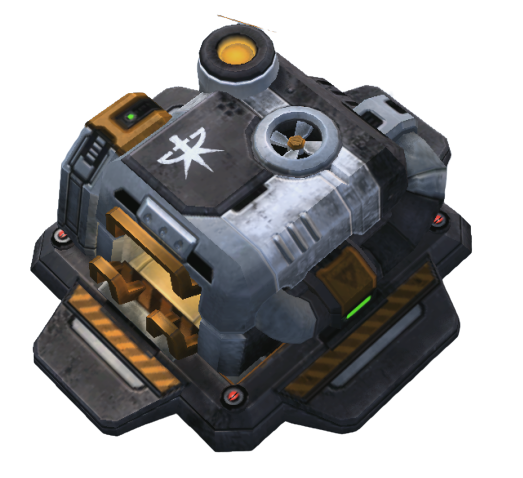
\includegraphics[width=\linewidth]{Figures/depot.png}
    \caption*{Supply Depot}\label{fig:depot}
    \endminipage\hfill
    \minipage{0.30\textwidth}
    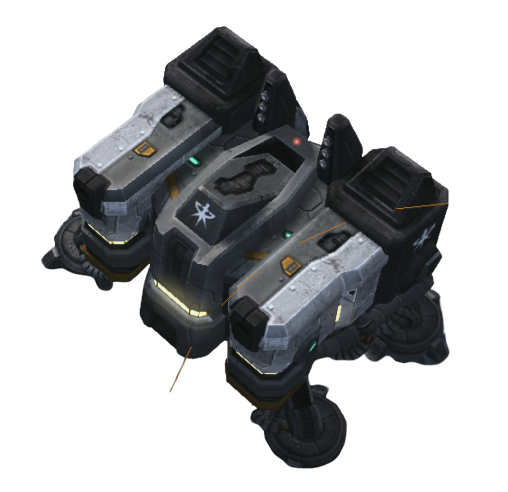
\includegraphics[width=\linewidth]{Figures/barracks.png}
    \caption*{Barracks}\label{fig:barracks}
    \endminipage\hfill
    \minipage{0.26\textwidth}
    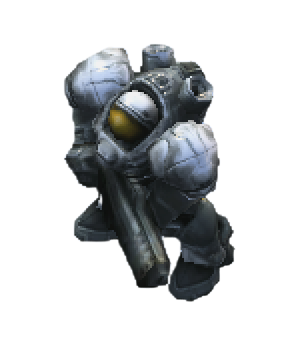
\includegraphics[width=\linewidth]{Figures/marine.png}
    \caption*{Marine}\label{fig:marine}
    \endminipage
    \caption{Dependency chain}
\end{figure}
So the agent has to recognize the dependency chain of Marine, Barracks and Supply Depot, see figures \ref{fig:depot} to \ref{fig:marine}. In past experiments with reinforcement learning agents, it was difficult to recognize this complex relationship. Most known algorithms were not able to successfully learn Montezuma's revenge from the Atari 2060 collection, see \cite{DBLP:journals/corr/abs-1805-11592}. What distinguishes Montezuma's Revenge from other Atari games is its relatively sparse rewards. The agent only receives rewards after completing a specific series of actions of extended periods of time. DeepMind reveals in their online blog, that their initial investigations showed that their agents performed well on the mini-games offered by the SC2LE \cite{DeepMindBlog2017}.
A similar challenge is proposed by our simplified StarCraft II scenario, which leads to the findings from the experiments we made.

\subsection{Performance - hactar}
The experimental reinforcement learning tasks have been held on the {\it hactar} scientific calculus system provided by the Technical University of Cologne. It features a Intel(R) Xeon(R) CPU E5-2680 v4 clocked at 2.40GHz with 56 logical cores and 256 GB Random Access Memory (RAM). Ubuntu Linux 16.04.6 LTS is used as operating system. Hactar also contains two high performance Graphics Processing Units (GPU) to further accelerate some calculations. By using the hactar system we can run the environment faster than real time. Observations are rendered at a speed that depends on several factors. For our simple optimization scenario the world simulation is very fast, so rendering the observation is the most critical part. This usually means the Python interpreter becomes the bottleneck. Possible gains by running over 4 parallel threads with a single interpreter are negated by that bottleneck, see \cite{DBLP:journals/corr/abs-1708-04782}.
\subsection{Training and Stability}
When using supervised learning, we can easily track the performance of a model during training by using the training and validation datasets for evaluation. In reinforcement learning accurately evaluating the progress of an agent during training can be challenging. The evaluation metric we use is the total reward accumulated by our test agents over the course of an episode or game averaged over a number of games. This mean reward is calculated periodically while training. Training stability has been very good for both DQN and ApeX, however, we had to skip the A3C for this project due to exploding gradients during training.
\subsection{Results}\label{sec:results}
Looking at the course of the average reward the agents managed to receive 
\subsection{Learnings}
\subsection{Related Work}
Initially, this work was part of a postgraduate project trying to enable agents to competitively play StarCraft using reinforcement learning. As of today, the focus of the dissertation has shifted towards the automated hyper-parameter tuning using so-called {\it meta learners}, researched by M.Sc. Jan Bollenbacher.
Tied closely to this work, fellow student Florian Soulier has studied how changing DQN agents parameter sets influence their performance using a grid search on different settings. In the context of using artificial intelligence with StarCraft fellow student Omar Kemachem studied clustering of StarCraft player strategies by looking at frames of the game replays provided by the SC2LE. 
\section{Conclusion}
In this project we set up a simple optimization scenario that can be solved by a human player fairly quick. We had different reinforcement learning algorithms trained to the set up environment, coming up with rather poor results. The results indicate that the simpler algorithms are not capable of learning the time delayed dependency chains they face in our scenario. Looking forward, one should focus on the more complex algorithms, considering especially the use of LSTM and transformers to depict these dependency chains.
\begin{appendix}
    \listoffigures
    \listoftables
    
\end{appendix}
\bibliographystyle{abbrvdin}
\bibliography{researchProject}
\end{document}
